
\documentclass{bredelebeamer}

\usepackage{color}
\usepackage{xcolor}
\usepackage{soul}
\definecolor{mGreen}{rgb}{0,0.6,0}
\definecolor{mGray}{rgb}{0.5,0.5,0.5}
\definecolor{mPurple}{rgb}{0.58,0,0.82}
\definecolor{backgroundColour}{rgb}{0.95,0.95,0.92}
\usepackage{colortbl}
\definecolor{Light}{gray}{.90}
\sethlcolor{Light}


\usepackage{amsmath}

\usepackage{algorithmicx}
\usepackage{algpseudocode}
\usepackage{parcolumns}
\usepackage{lipsum}

\usepackage{listings}

\lstdefinestyle{CStyle}{
    backgroundcolor=\color{backgroundColour},
    commentstyle=\color{mGreen},
    keywordstyle=\color{magenta},
    numberstyle=\tiny\color{mGray},
    stringstyle=\color{mPurple},
    basicstyle=\scriptsize,
    %basicstyle=\tiny,
    breakatwhitespace=false,
    breaklines=true,
    captionpos=t,
    keepspaces=true,
    numbers=left,
    numbersep=5pt,
    showspaces=false,
    showstringspaces=false,
    showtabs=false,
    tabsize=2,
    language=C
}

\lstdefinestyle{customasm}{
  backgroundcolor=\color{backgroundColour},
  belowcaptionskip=1\baselineskip,
  frame=L,
  xleftmargin=\parindent,
  language=[x86masm]Assembler,
  basicstyle=\footnotesize\ttfamily,
  commentstyle=\itshape\color{purple!40!black},
}

\usepackage{placeins}

\usepackage{parskip}
%%%%%%%%%%%%%%%%%%%%%%%%%%%%%%%%%%%%%%%%%%%%%%%%



\title[Calcul du flux optique sur Raspbery Pi]{Implémentation embarquée d'un algorithme de calcul de flux optique sur un dr\^one sous-marin autonome}
% Titre du diaporama

\subtitle{Processeur Graphique \textsc{VideoCore IV 3D}}
% Sous-titre optionnel

\author{Simon Bataille\inst{1}}
% La commande \inst{...} Permet d'afficher l' affiliation de l'intervenant.
% Si il y a plusieurs intervenants: Marcel Dupont\inst{1}, Roger Durand\inst{2}
% Il suffit alors d'ajouter un autre institut sur le modèle ci-dessous.

\institute[Université de Caen Normandie]
{
  \inst{1}%
  ESIX NORMANDIE\\
  Département Mécatronique \& Systèmes Nomades
  }


\date{28 Septembre 2018}
% Optionnel. La date, généralement celle du jour de la conférence

\subject{Stage de fin d'étude}
% C'est utilisé dans les métadonnes du PDF



\logo{

\includegraphics[scale=0.3]{images/logoNotilo.png}
}



%%%%%%%%%%%%%%%%%%%%%%%%%%%%%%%%%%%%%%%%%%%%%%%%%%%%%%%%%%%%%%%%%%%%%
\begin{document}

\begin{frame}
  \titlepage
\end{frame}





\begin{frame}{Sommaire}
  \tableofcontents
  % possibilité d'ajouter l'option [pausesections]
\end{frame}




%%%%%%%%%%%%%%%%%%%%%%%%%%%%%%%%%%%%%%%%%%%%%%%%%%%%%%%%%%%%%%%%%%%%%
%%%%%%%%%%%%%%%%%%%%%%%%%%%%%%%%%%%%%%%%%%%%%%%%%%%%%%%%%%%%%%%%%%%%%

\section{Introduction}

%%%%%%%%%%%%%%%%%%%%%%%%%%%%%%%%%%%%%%%%%%%%%%%%%%%%%%%%%%%%%%%%%%%%%

	\subsection{Notilo+ \& iBubble}

%--------------------------------------------------------------------

\begin{frame}{Entreprise d'accueil : Notilo+}

\begin{itemize}
\item Jeune start-up créée à Lyon en 2016
\item Développement d'un dr\^one sous-marin autonome: iBubble
\begin{figure}
\centering
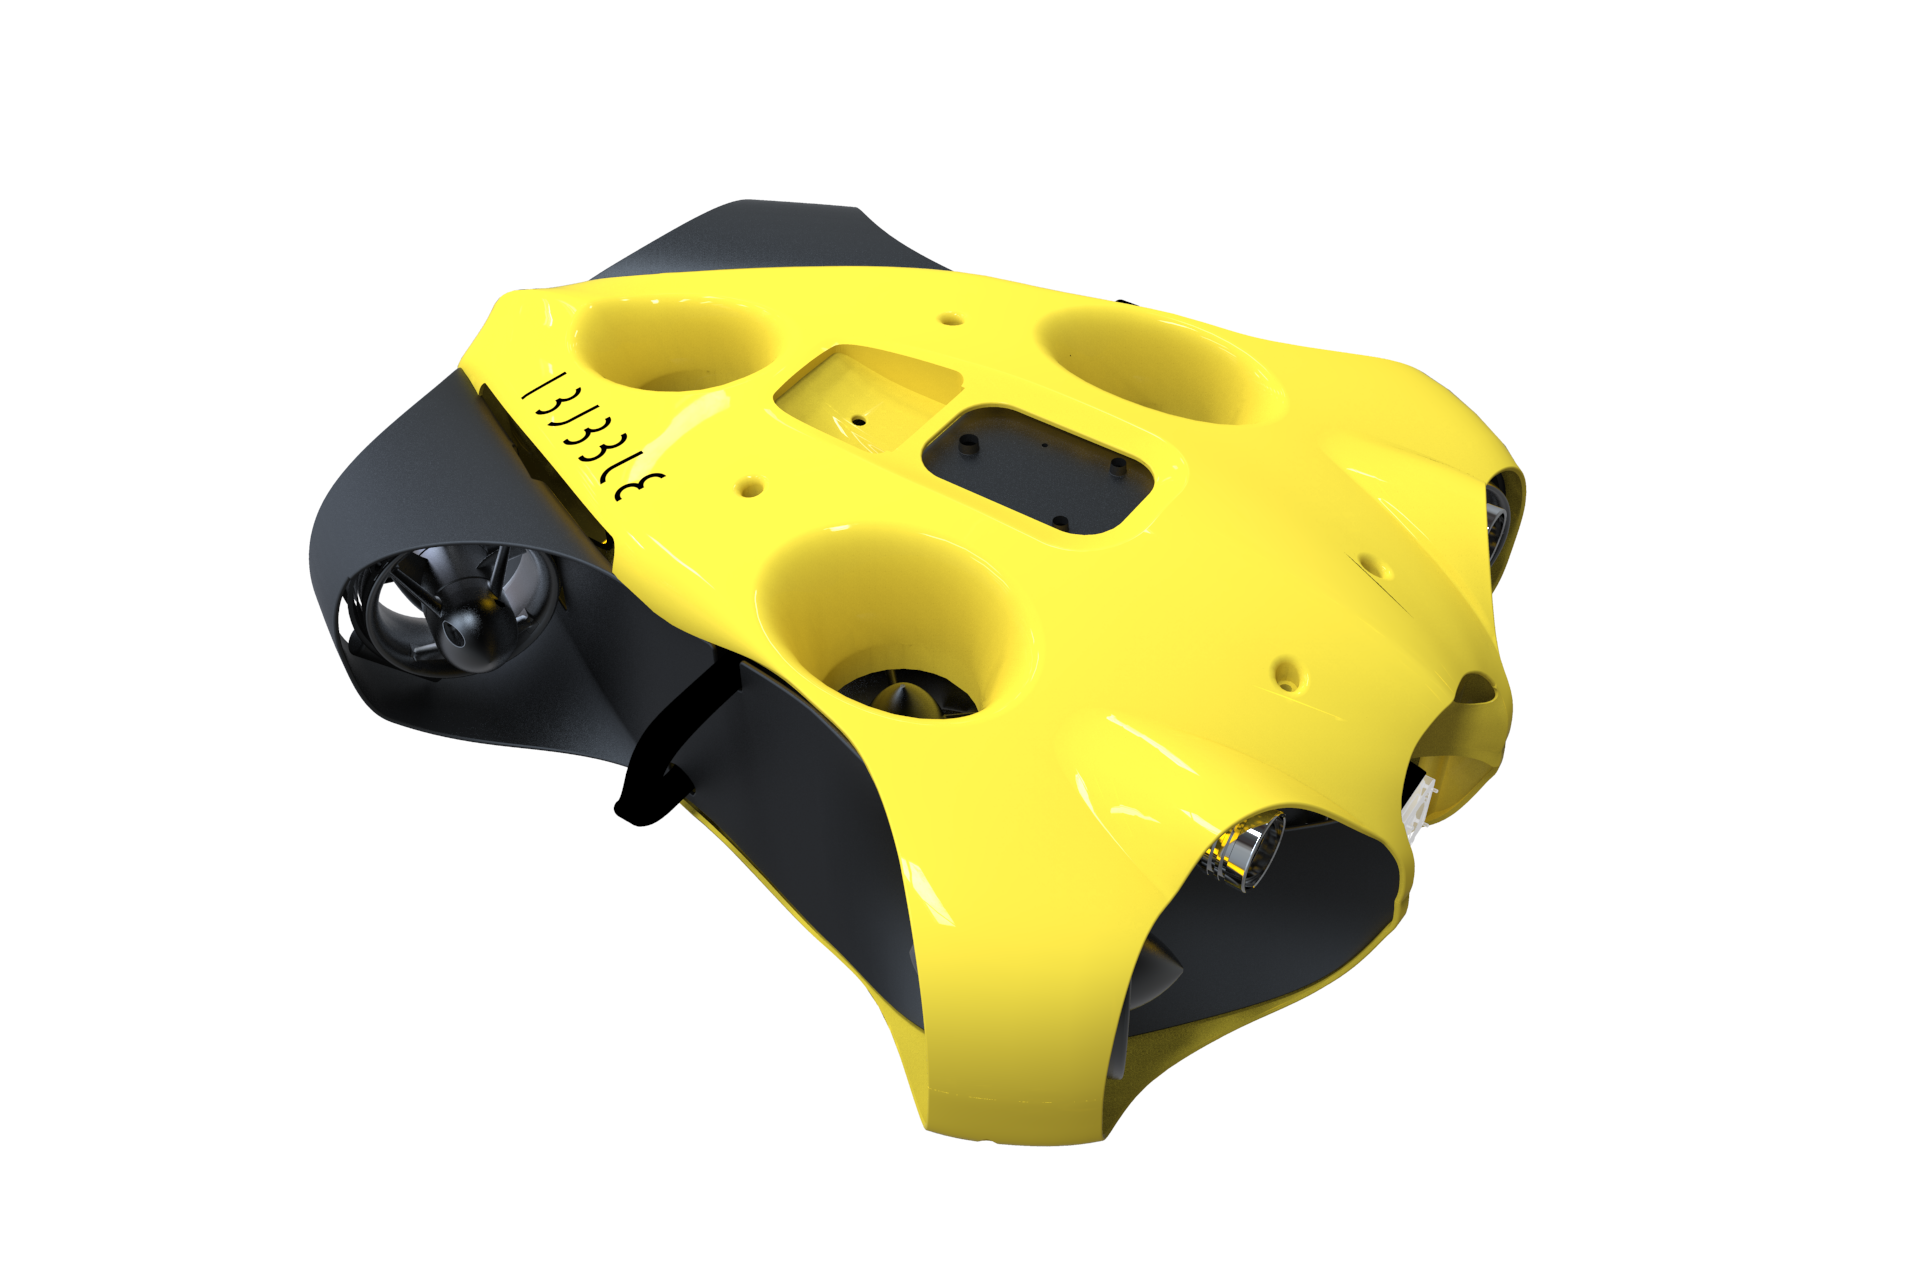
\includegraphics[scale=0.05]{images/iBubble3.png}
\caption{iBubble}
\end{figure}
\item Environ 25 personnes réparties en 2 équipes:
	\begin{itemize}
	\item équipe commerciale
	\item équipe technique
	\end{itemize}
\item Tuteur: Filip Novotny -- responsable de la partie vision
\item Thibault Anquetil -- ancien élève à l'ESIX
\end{itemize}

\end{frame}

%--------------------------------------------------------------------

\begin{frame}{iBubble}

\begin{block}{Caractéristiques}
\begin{itemize}
\item Aquatique et Autonome
\item Repérage Acoustique
\item Système de Suivi Visuel
\end{itemize}
\end{block}

\begin{block}{Développement}
\begin{itemize}
\item Hardware: mécanique et conception électronique
\item Embarquée: logiciel pilotant iBubble
\item Informatique haut niveau: algorithmes de suivi par vision
\end{itemize}
\end{block}

\end{frame}

%--------------------------------------------------------------------

%%%%%%%%%%%%%%%%%%%%%%%%%%%%%%%%%%%%%%%%%%%%%%%%%%%%%%%%%%%%%%%%%%%%%

	\subsection{Problématique \& Réponse}

%--------------------------------------------------------------------

\begin{frame}{Problématique}

\begin{block}{Algorithme de tracking visuel}
\begin{itemize}
\item CMT -- algorithme de suivi visuel bien connu
\item Initialement, iBubble développé avec une carte Jetson
\begin{itemize}
\item GPGPU à architecture CUDA
\item Optimisation du CMT à 30 images par seconde
\end{itemize}
\end{itemize}
\end{block}

\begin{block}{Raspberry Pi}
\begin{itemize}
\item Carte embarquée sur la version commerciale de iBubble
\item SoC BCM2837 -- BROADCOM
\begin{itemize}
\item CPU -- ARM
\item GPU VideoCore IV 3D -- BROADCOM
\end{itemize}
\item Pas une architecture CUDA
\begin{itemize}
	\item Pas d'optimation du CMT
	\item VideoCore inutilisé
	\item 7 images par seconde
\end{itemize}
\end{itemize}
\end{block}

\end{frame}

%--------------------------------------------------------------------

\begin{frame}{Réponse}
\begin{block}{Flux optique}
\begin{itemize}
\item Calcul du Flux Optique
\begin{itemize}
	\item Partie du CMT qui consomme le plus de ressources
	\item Parallèlisable sur GPU
\end{itemize}
\item Implémentation interne du calcul du Flux Optique
\item Utilisation du GPU de la Rasperry Pi pour certains calculs
\end{itemize}
\end{block}

\begin{exampleblock}{Tâches}
\begin{itemize}
\item Comprendre l'archtecture du VideoCore IV 3D
\item Apprendre à programmer le VideoCore IV 3D
\item Implémenter le calcul du Flux Optique sur Raspberry Pi
\end{itemize}
\end{exampleblock}

\begin{alertblock}{Difficultés}
\begin{itemize}
\item Aucune API officielle éxistante pour l'utilisation du VideoCore IV 3D
\item Programmation en assembleur à partir de projets non-officiels
\end{itemize}
\end{alertblock}

\end{frame}

%--------------------------------------------------------------------



%%%%%%%%%%%%%%%%%%%%%%%%%%%%%%%%%%%%%%%%%%%%%%%%%%%%%%%%%%%%%%%%%%%%%
%%%%%%%%%%%%%%%%%%%%%%%%%%%%%%%%%%%%%%%%%%%%%%%%%%%%%%%%%%%%%%%%%%%%%

\section{Sujet}

%%%%%%%%%%%%%%%%%%%%%%%%%%%%%%%%%%%%%%%%%%%%%%%%%%%%%%%%%%%%%%%%%%%%%

	\subsection{Flux Optique}


%--------------------------------------------------------------------

\begin{frame}{Données entrantes: que traite-t-on ?}


\begin{block}{Images issues de la RaspiCam}
\begin{itemize}
\item Matrices $240\times 360$ -- floats 32-bit $\in \left[0;1\right]$
\item Lignes contigues en RAM -- Row-major
\item Adressage 32-bit
\end{itemize}
\end{block}

\begin{figure}
\centering
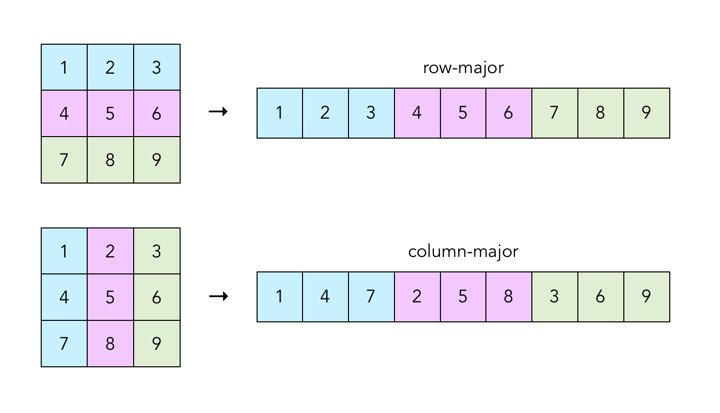
\includegraphics[scale=0.2]{images/rowcolumnarrays.jpg}
\caption{Stockage des pixels en RAM}
\end{figure}


\end{frame}

%--------------------------------------------------------------------

\begin{frame}{Données entrantes: que traite-t-on ?}


\begin{block}{Features}
\begin{itemize}
\item Points d'intér\^ets encadrants le plongeur
\item Utiliser dans le CMT pour suivre le plongeur
\item Repérées par le couple $(x,y)$:
	\begin{itemize}
		\item $x$ -- ligne de la feature $\in \left[0;240\right]$
		\item $y$ -- colonne de la feature $\in \left[0;360\right]$
	\end{itemize}
\end{itemize}
\end{block}

\begin{figure}
\centering
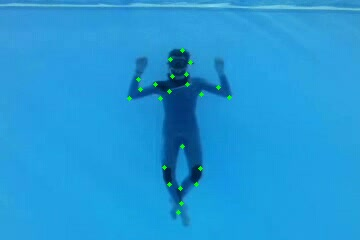
\includegraphics[scale=0.5]{images/plongeurInitFeatures.jpeg}
\end{figure}


\end{frame}

%--------------------------------------------------------------------

\begin{frame}{Flux Optique}

\begin{alertblock}{Flux Optique}
Déplacemensubt de ces features entre 2 images consécutives d'une vidéo
\begin{itemize}
	\item $d_{x}$: déplacement de la feature suivant les lignes
	\item $d_{y}$: déplacement de la feature suivant les colonnes
	\item Déplacements mesurés en pixels
\end{itemize}
\end{alertblock}

\begin{figure}
\centering
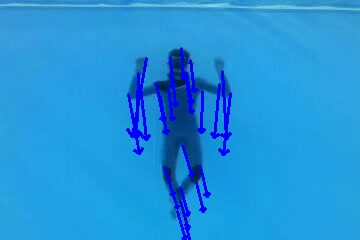
\includegraphics[scale=0.4]{images/plongeurOpticalFlow.jpeg}
\caption{Flux optique entre les 2 images}
\end{figure}

\end{frame}

%--------------------------------------------------------------------

\begin{frame}{Flux Optique entre 2 images successives}

\begin{columns}
\begin{column}{0.3\textwidth}
\begin{figure}
\centering
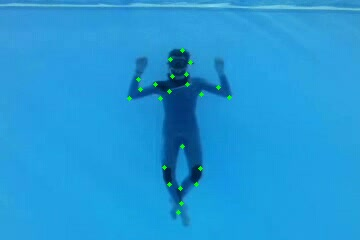
\includegraphics[scale=0.3]{images/plongeurInitFeatures.jpeg}
\caption{FEATURES sur la première image}
\end{figure}
\end{column}


\begin{column}{0.3\textwidth}
\begin{figure}
\centering
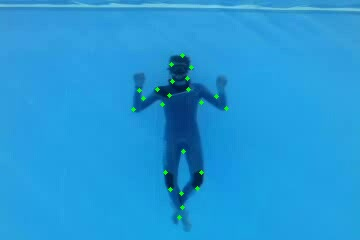
\includegraphics[scale=0.3]{images/plongeurNextFeatures.jpeg}
\caption{FEATURES sur la deuxième image}
\end{figure}
\end{column}

\end{columns}

%\begin{column}{0.3\textwidth}
\begin{figure}
\centering
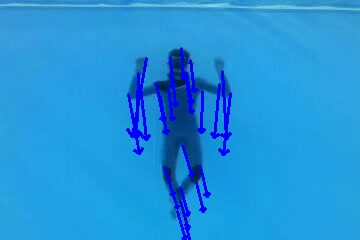
\includegraphics[scale=0.3]{images/plongeurOpticalFlow.jpeg}
\caption{Flux optique entre les 2 images}
\end{figure}
%\end{column}

%\end{columns}

\end{frame}

%--------------------------------------------------------------------

\begin{frame}{Flux Optique : $x_{2}=x_{1}+d_{x}$, $y_{2}=y_{1}+d_{y}$}

\begin{figure}
%\centering
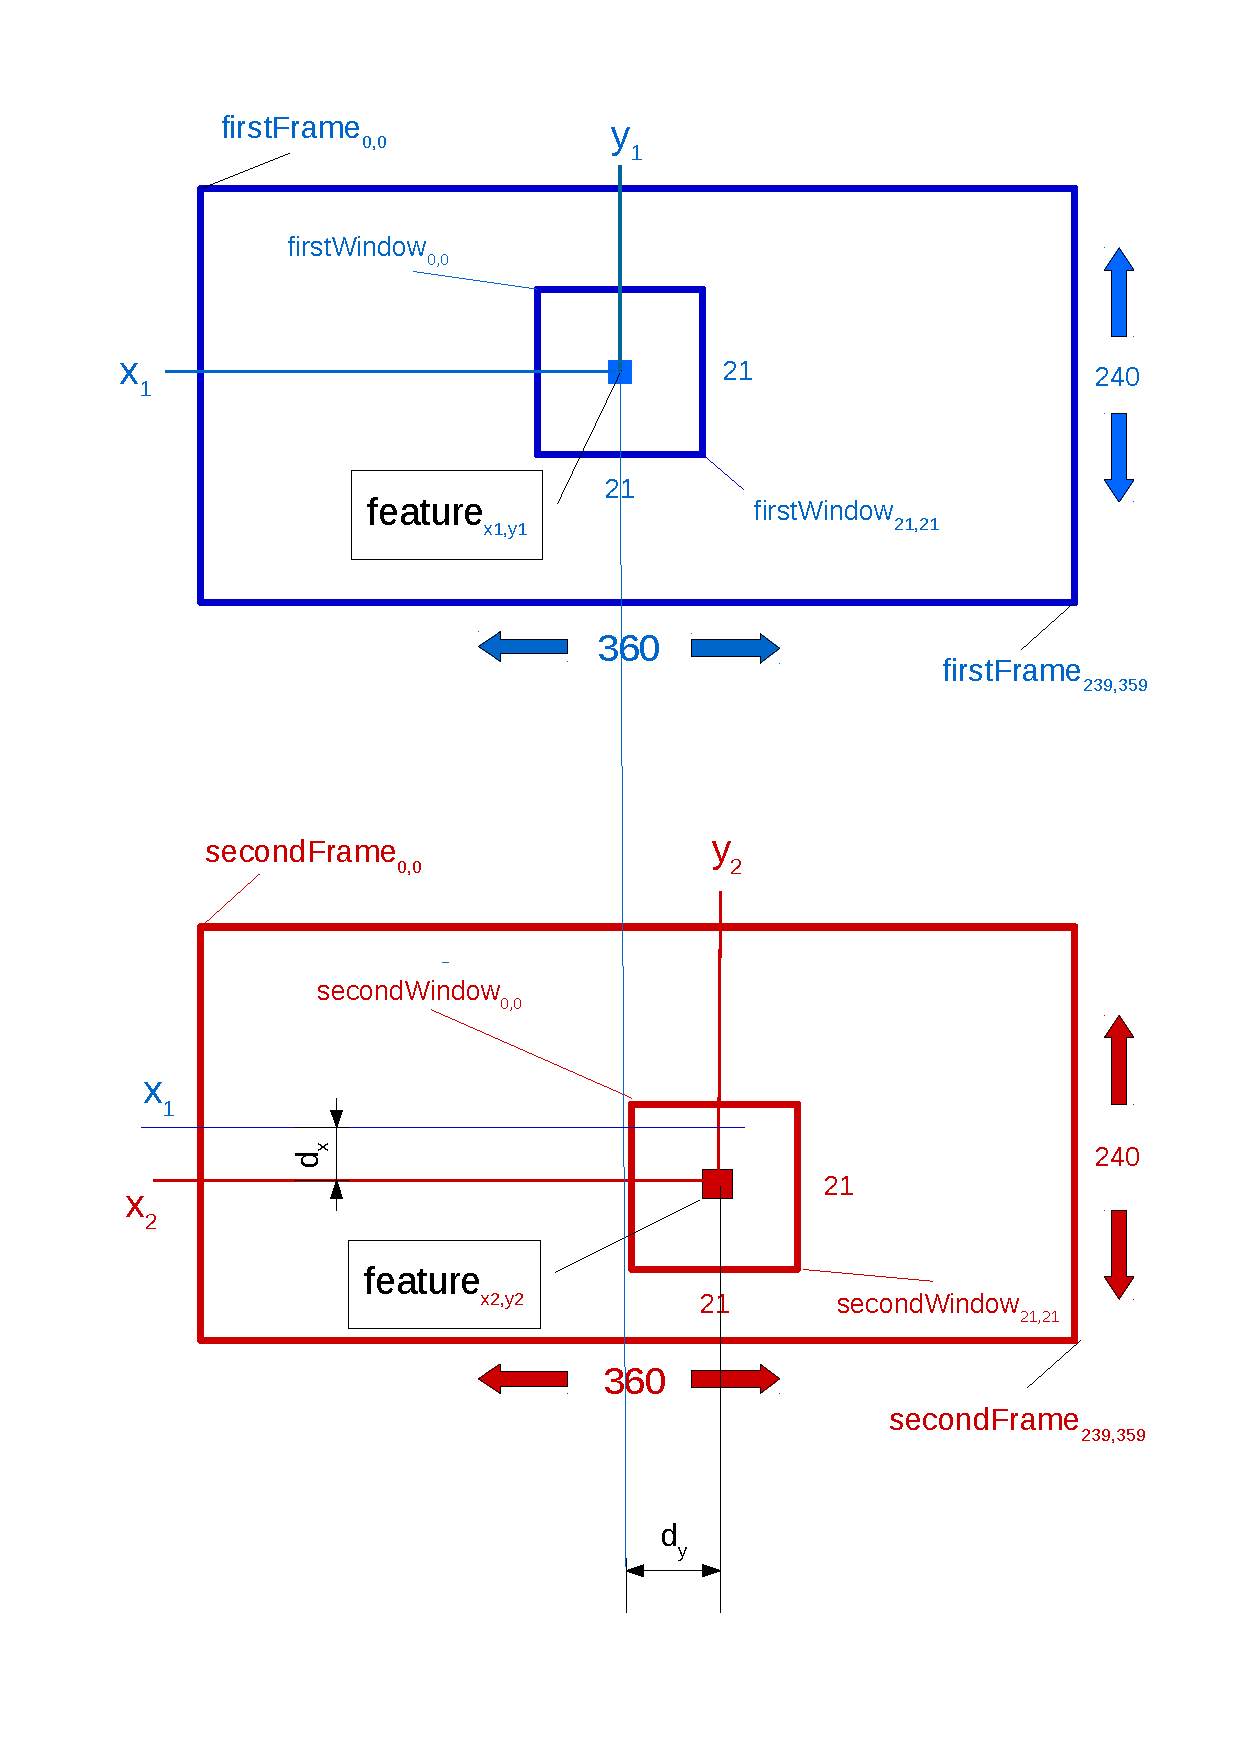
\includegraphics[scale=0.3]{images/framesWindow.pdf}
\end{figure}

\end{frame}

%--------------------------------------------------------------------

%%%%%%%%%%%%%%%%%%%%%%%%%%%%%%%%%%%%%%%%%%%%%%%%%%%%%%%%%%%%%%%%%%%%%

\subsection{Méthode de Lucas-Kanade}

%--------------------------------------------------------------------

\begin{frame}{Méthode de Lucas-Kanade}

\begin{block}{Estimation du Flux Optique pour chaque FEATURE}
\begin{itemize}
	\item Plusieurs algorithmes permettant le calcul
	\item Camille a sélectionné la Méthode de Lucas-Kanade -- Algorithme bien connu
	\item Entre 2 images successives
\end{itemize}
\end{block}

\begin{exampleblock}{2 Etapes}
\begin{itemize}
	\item Première étape dite de Gradient sur la première image
	\item Deuxième étape du calcul effectif du flux optique pour chaque FEATURE
	\item 30 FEATURES sur l'image -- 1 seule FEATURE
\end{itemize}
\end{exampleblock}

\end{frame}

%--------------------------------------------------------------------

\begin{frame}{Gradient sur la première image pour une FEATURE}

	\begin{block}{4 Valeurs à calculer}
\begin{itemize}
	\item $G_{XX}$ -- gradient vertical de la FEATURE
	\item $G_{YY}$ -- gradient horizontal de la FEATURE
	\item $G_{XY}$ -- gradient croisé de la FEATURE
	\item $det = \frac{1}{G_{XX}G_{YY}-G_{XY}G_{XX}}$
\end{itemize}
\end{block}


\boitejaune{
	$$G_{YY} = \sum_{i=1}^{21}\sum_{j=1}^{21} grad_{y}[i,j]^{2}$$\\
	$$G_{XY} = \sum_{i=1}^{21}\sum_{j=1}^{21} grad_{x}[i,j]\times grad_{y}[i,j]$$\\
	$$G_{XX} = \sum_{i=1}^{21}\sum_{j=1}^{21} grad_{x}[i,j]^{2}$$
}

\end{frame}

%--------------------------------------------------------------------

\begin{frame}{Gradient sur la première image pour une FEATURE}

	\begin{block}{Fen\^etre autour de la FEATURE}
 $$grad_{x}[i,j] = \frac{\textcolor{blue}{firstWindow_{i+1,j}} - \textcolor{blue}{firstWindow_{i-1,j}}}{2}$$
 $$grad_{y}[i,j] = \frac{\textcolor{blue}{firstWindow_{i,j+1}} - \textcolor{blue}{firstWindow_{i,j-1}}}{2}$$
\end{block}

\begin{figure}
\centering
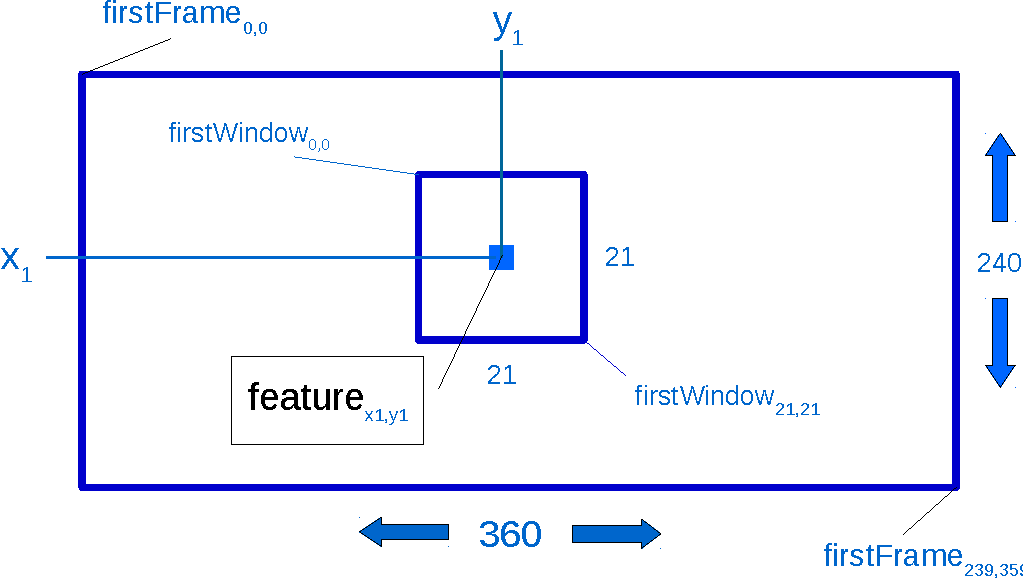
\includegraphics[scale=0.3]{images/firstFrameWindow.pdf}
\end{figure}

\end{frame}

%--------------------------------------------------------------------

\begin{frame}{Flux Optique: $d_{x}, d_{y}$}

	\begin{block}{Algorithme de calcul du déplacement -- Plusieurs itérations -- Valeurs initiales nulles}
\begin{algorithmic}
	\ForAll {$\textcolor{blue}{firstWindow_{i,j}}$ and $\textcolor{red}{secondWindow_{i,j}}$}

	\State $diff\_frames = \textcolor{blue}{firstWindow_{i,j}} - \textcolor{red}{secondWindow_{i+d_{x},j+d_{y}}}$

	\State $frames\_mismatch.x = diff\_frames\times grad_{x}[i,j]$
	\State $frames\_mismatch.y = diff\_frames\times grad_{y}[i,j]$

	\EndFor

	\State $d_{x} = det\times (G_{YY}\times frames\_mismatch.x - G_{XY}\times frames\_mismatch.y)$
	\State $d_{y} = det\times (G_{XX}\times frames\_mismatch.y - G_{XY}\times frames\_mismatch.x)$
\end{algorithmic}
\end{block}

	\begin{alertblock}{Interpolation Bilinéaire}
\begin{equation*}
	\begin{split}
		\textcolor{red}{secondWindow_{i+d_{x},j+d_{y}}} =\\
		\textcolor{red}{secondWindow_{floor(i+d_{x}),floor(j+d_{y})}}\times (1-fract(i+d_{x}))\times (1-fract(i+d_{y}))\\
		+ \textcolor{red}{secondWindow_{floor(i+d_{x})+1,floor(j+d_{y})}}\times (fract(i+d_{x}))\times (1-fract(i+d_{y}))\\
		+ \textcolor{red}{secondWindow_{floor(i+d_{x}),floor(j+d_{y})+1}}\times (1-fract(i+d_{x}))\times (fract(i+d_{y}))\\
		+ \textcolor{red}{secondWindow_{floor(i+d_{x})+1,floor(j+d_{y})+1}}\times (fract(i+d_{x}))\times (fract(i+d_{x}))
	\end{split}
\end{equation*}
	\end{alertblock}

\end{frame}

%--------------------------------------------------------------------

\begin{frame}{Flux Optique entre 2 images successives pour une seule FEATURE }

\begin{figure}
\centering
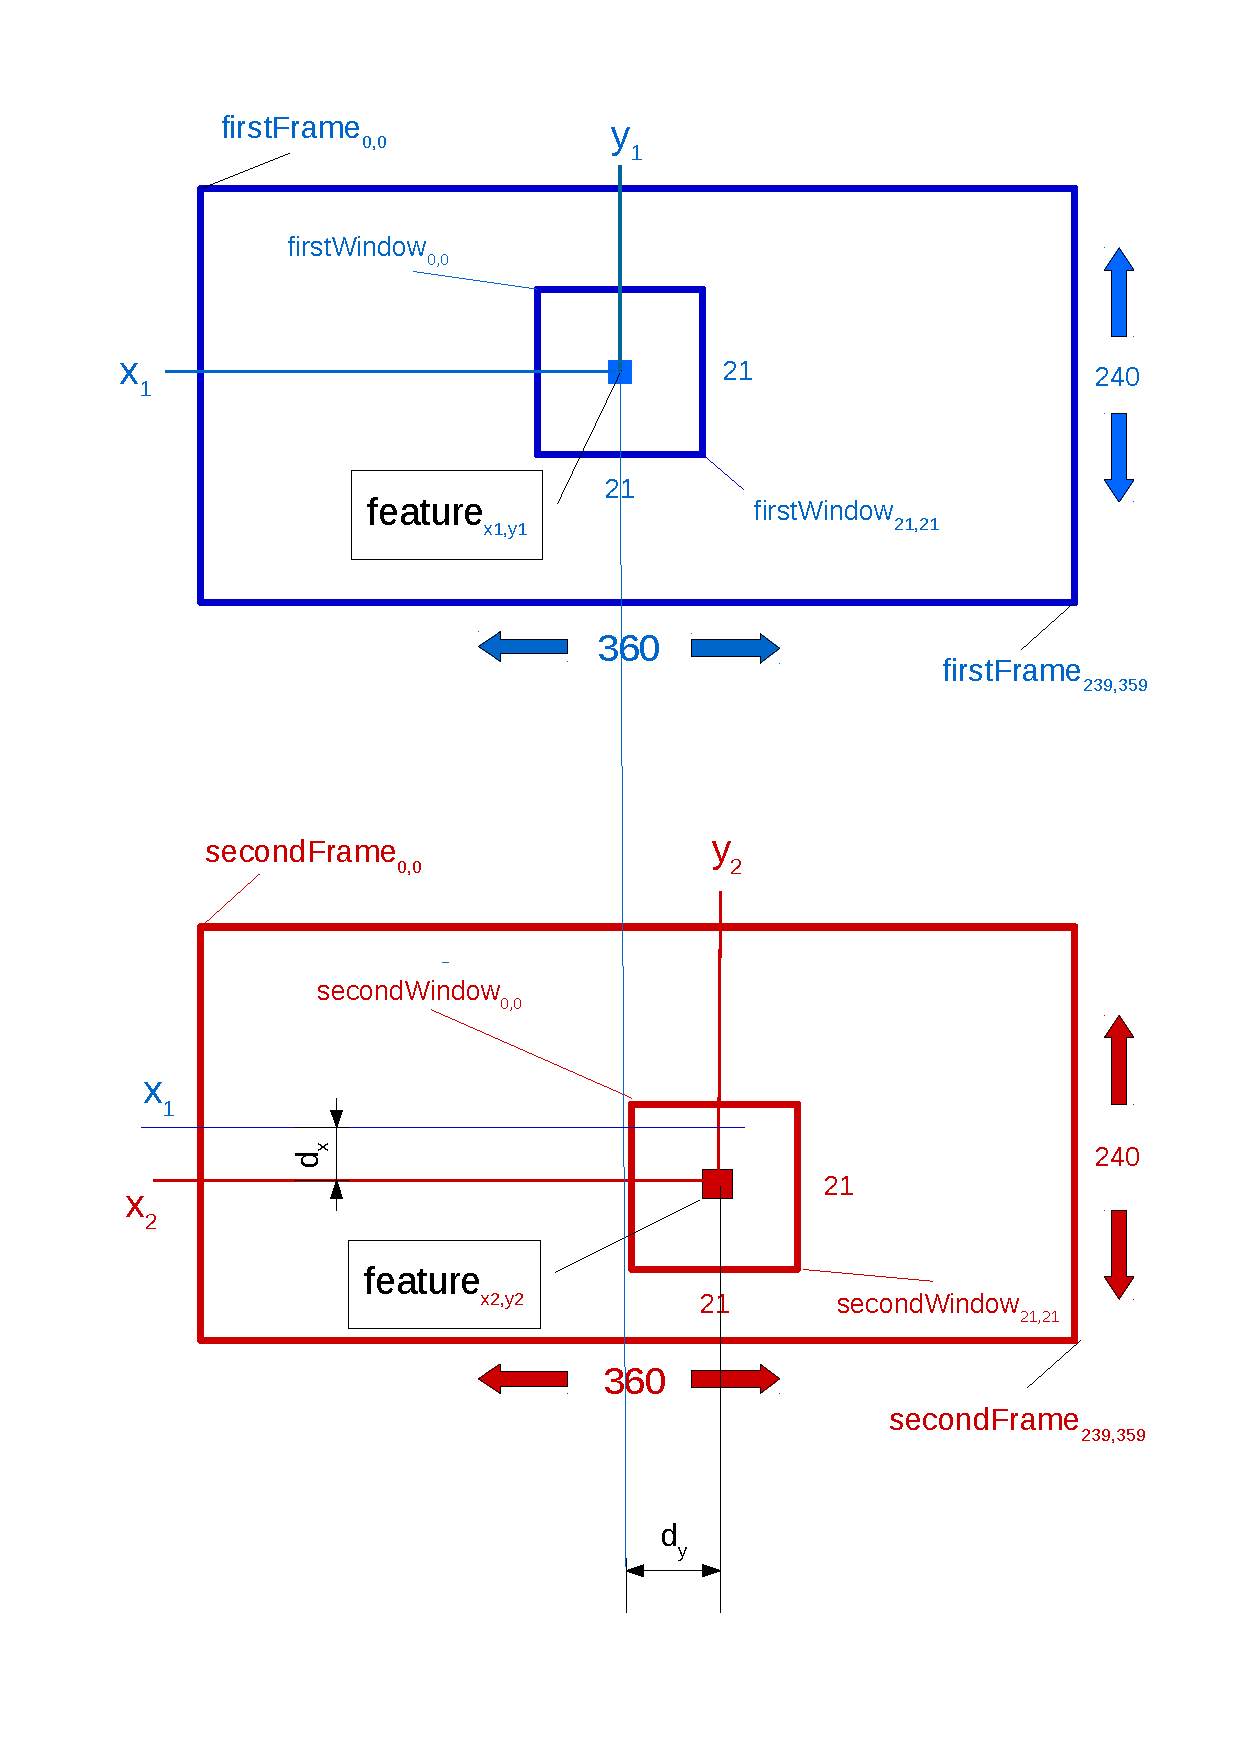
\includegraphics[scale=0.3]{images/framesWindow.pdf}
\end{figure}

\end{frame}

%--------------------------------------------------------------------

%%%%%%%%%%%%%%%%%%%%%%%%%%%%%%%%%%%%%%%%%%%%%%%%%%%%%%%%%%%%%%%%%%%%%

\subsection{VideoCore IV 3D}

%--------------------------------------------------------------------

\begin{frame}{GPU de la Raspberry Pi : VideoCore IV 3D}

\begin{block}{Documentation \& Caractérisques}
\begin{itemize}
\item Succès de la Raspberry Pi -- Documentation Officielle Broadcom
\item Vecteurs de 16 mots -- integer/float 32-bit
\item Jeu d'instructions -- add/fadd, mul24/fmul, branch, load, semaphore etc \ldots
\end{itemize}
\end{block}

\begin{block}{Apprentissage}
\begin{itemize}
\item Aucune API officielle
\item Projets indépendants sur github -- helloworld et pi-gemm
\item Parseurs d'assembleur -- Programmation en assembleur
\end{itemize}
\end{block}

\end{frame}

%--------------------------------------------------------------------

\begin{frame}{Programmation du VideoCore IV 3D}

\begin{alertblock}{Principes de programmation}
\begin{itemize}
\item GPU piloté par un CPU -- interface mailbox disponible sur le noyau Linux
	\begin{itemize}
		\item code à éxécuter sur GPU en assembleur puis parser
		\item driver en langage C éxécuter sur CPU pour envoyer le code et les variables
	\end{itemize}
\item Mémoire RAM partagée entre CPU \& GPUs -- 2 espaces d'adresses
	\begin{itemize}
		\item ARM Virtual Adresses -- CPU
		\item VC CPU Bus Adresses -- GPU
	\end{itemize}
\end{itemize}
\end{alertblock}

\end{frame}

%--------------------------------------------------------------------

\begin{frame}{Mémoire RAM partagée}

\begin{figure}
\centering
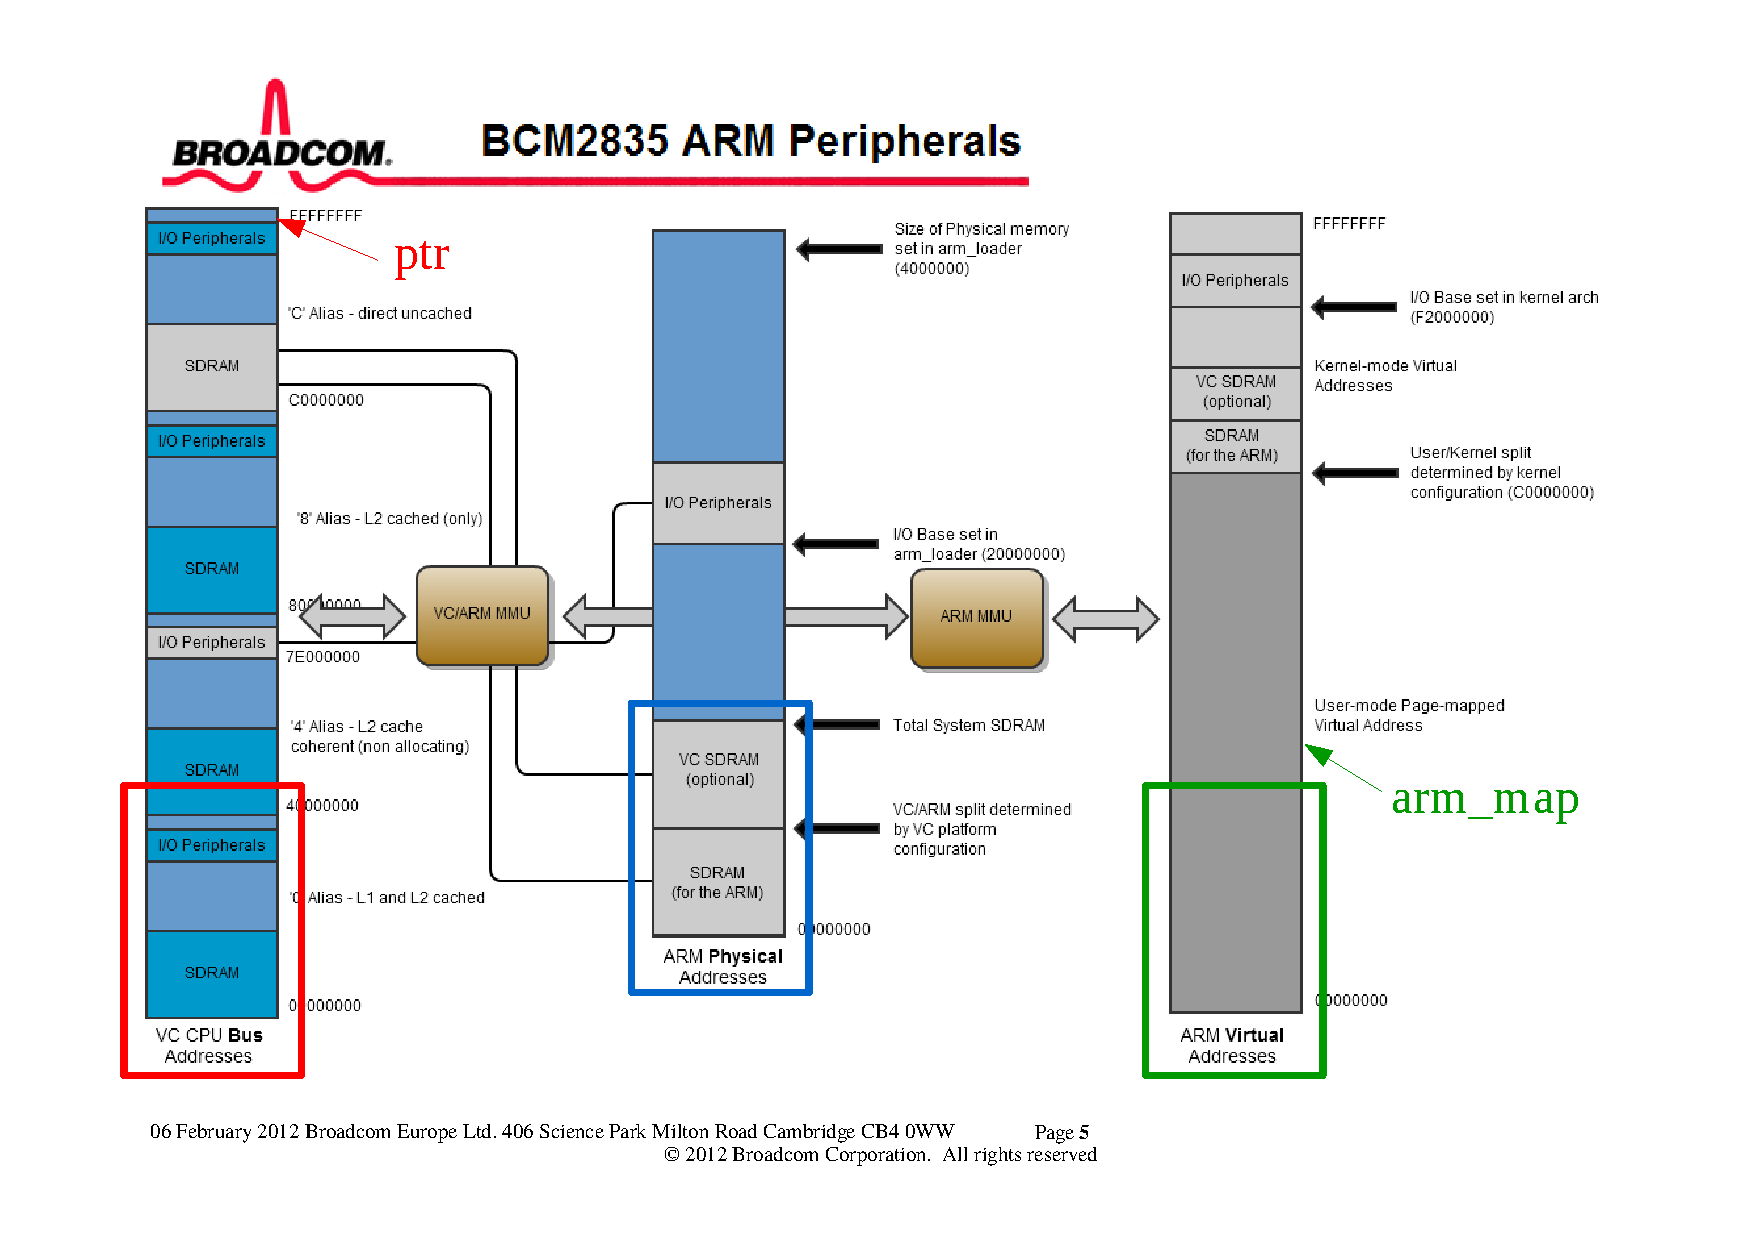
\includegraphics[scale=0.3]{images/RAMptrs.pdf}
\end{figure}

\end{frame}

%--------------------------------------------------------------------

\begin{frame}{Etapes de programmation}

\begin{block}{GPU}
\begin{enumerate}
\item Ecrire le code à éxécuter en assembleur
\item Parser ce code pour obtenir un fichier binaire compréhensible par le GPU
\end{enumerate}
\end{block}

\begin{block}{CPU}
\begin{enumerate}
\item Initialiser la RAM partagée
\item Copier en RAM le code à exécuter et les données entrantes (images et FEATURES)
\item Transmettre les pointeurs au GPU
\item Récupérer les résultats en RAM partagée
\end{enumerate}
\end{block}

\end{frame}

%-------------------------------------------------------------------

\begin{frame}{Architecture du GPU}

\begin{figure}
\centering
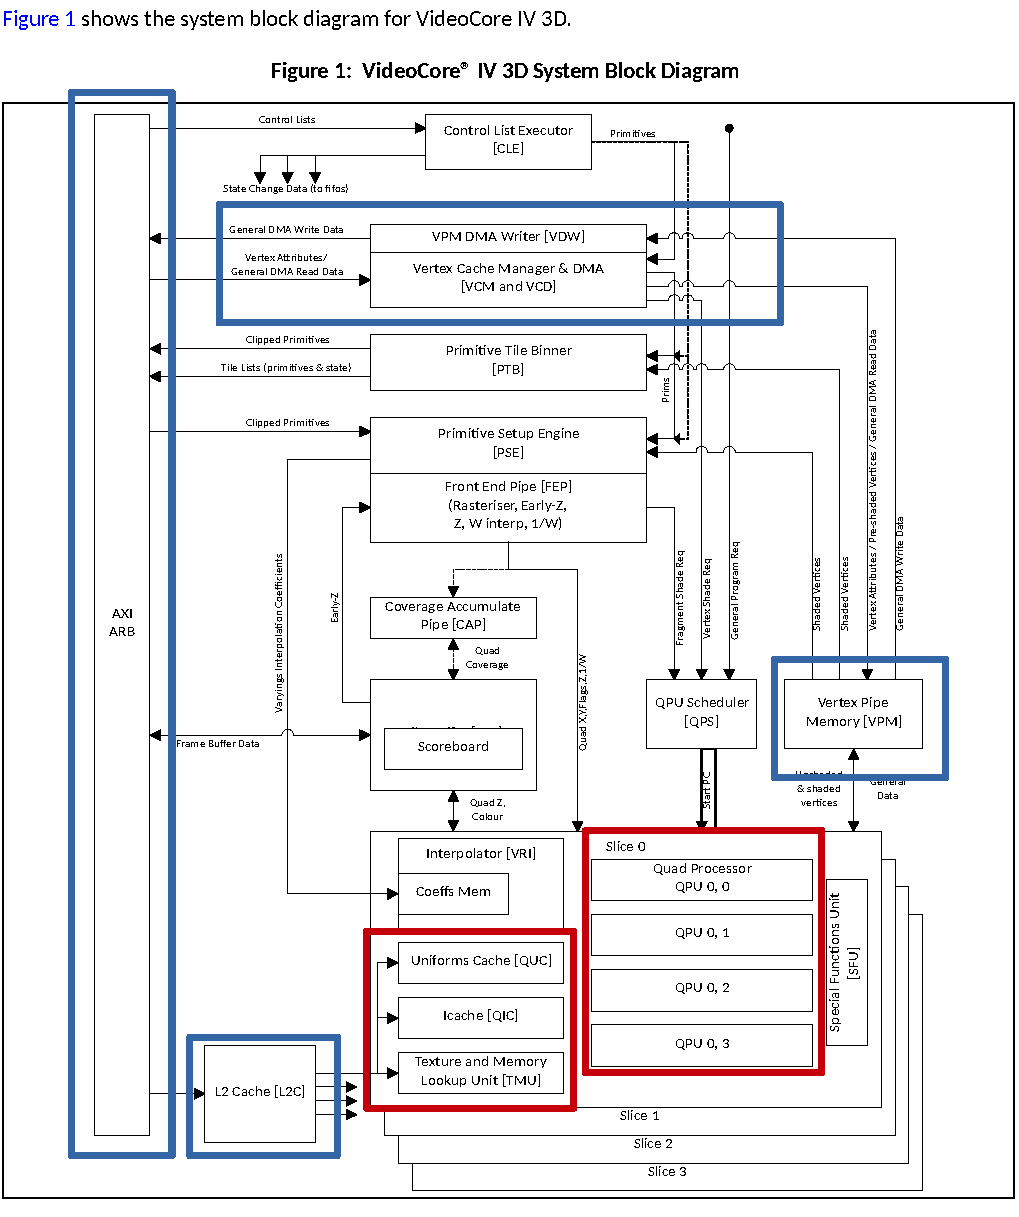
\includegraphics[scale=0.4]{images/archOverview.pdf}
\end{figure}

\end{frame}

%--------------------------------------------------------------------



%%%%%%%%%%%%%%%%%%%%%%%%%%%%%%%%%%%%%%%%%%%%%%%%%%%%%%%%%%%%%%%%%%%%%
%%%%%%%%%%%%%%%%%%%%%%%%%%%%%%%%%%%%%%%%%%%%%%%%%%%%%%%%%%%%%%%%%%%%%

\section{Solution}

%%%%%%%%%%%%%%%%%%%%%%%%%%%%%%%%%%%%%%%%%%%%%%%%%%%%%%%%%%%%%%%%%%%%%

\subsection{Bibliothèque interne}

%--------------------------------------------------------------------

\begin{frame}{Architecture du projet}

\begin{figure}
\centering
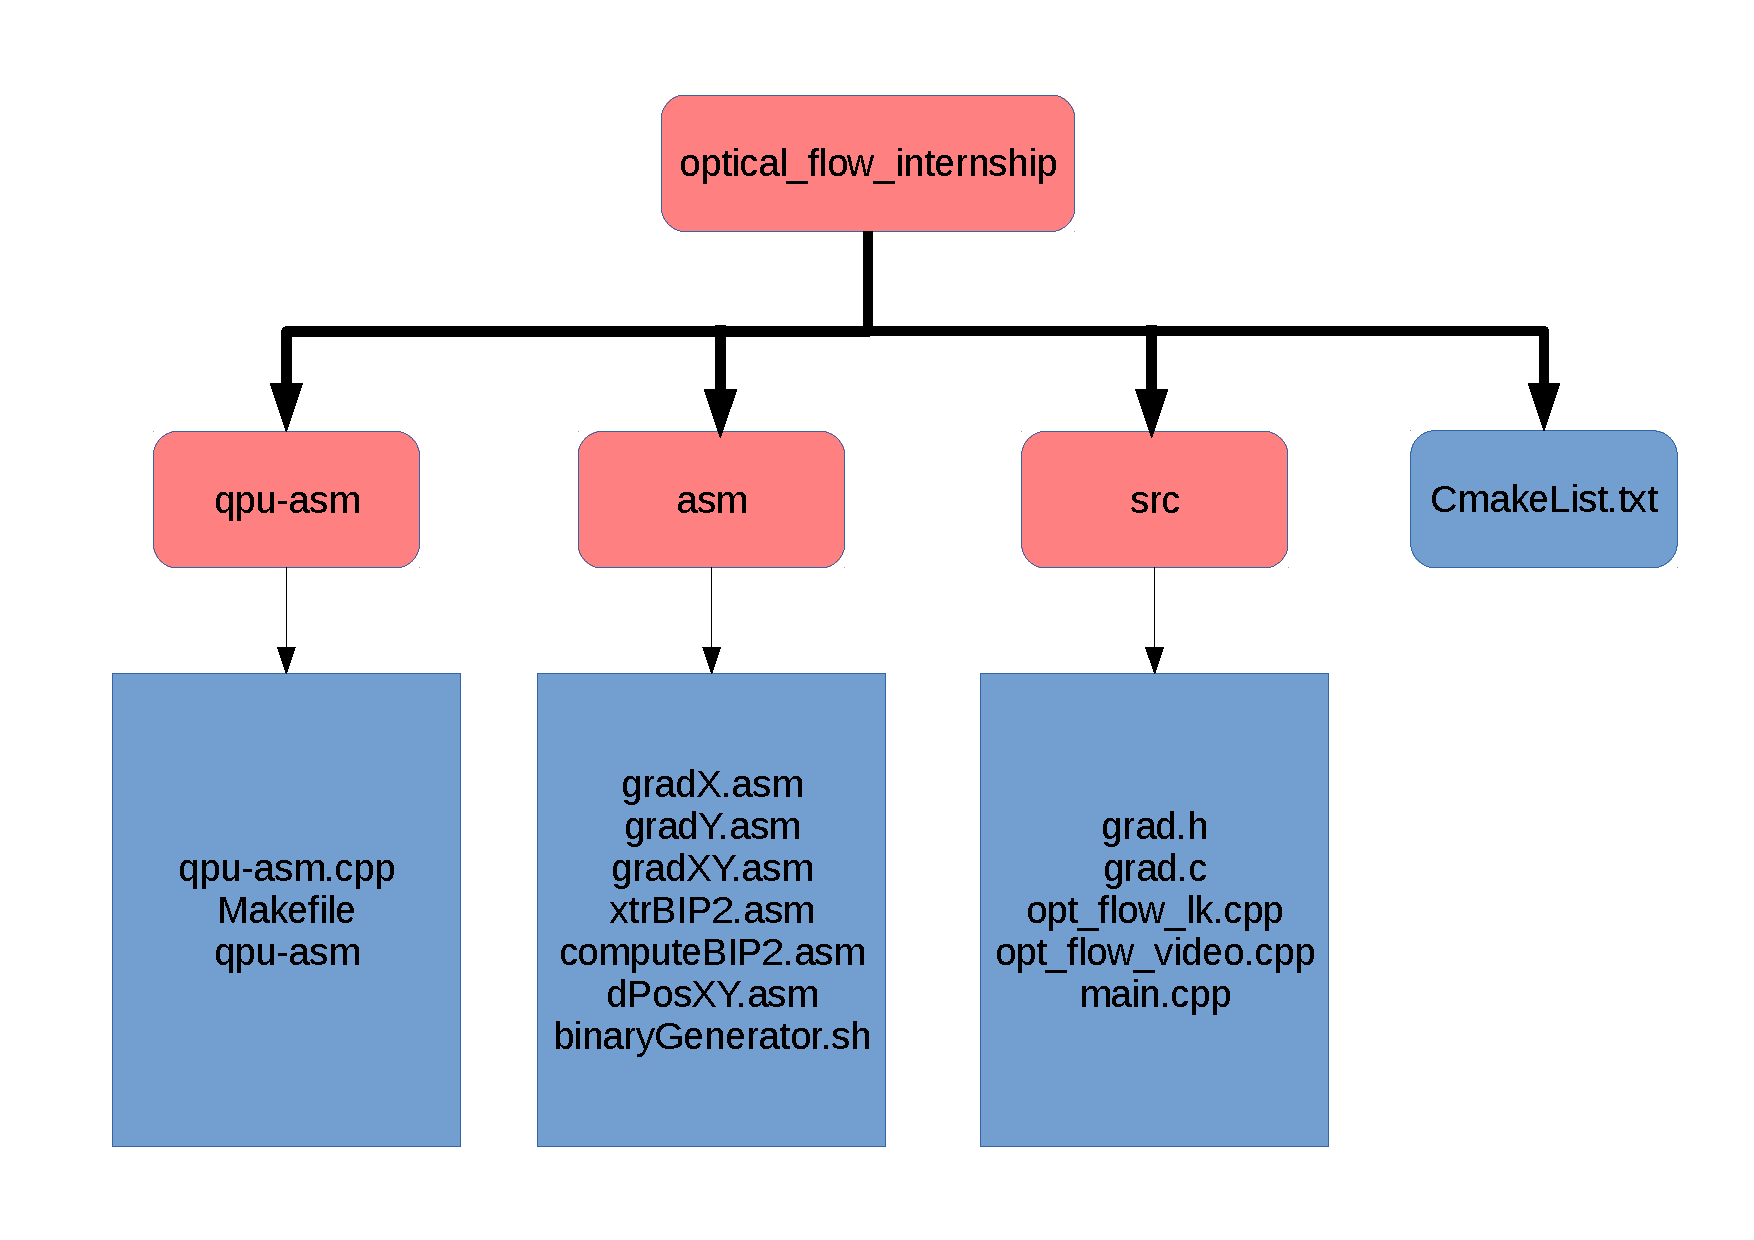
\includegraphics[scale=0.3]{images/optFlowArchitecture.pdf}
\end{figure}

\end{frame}

%--------------------------------------------------------------------

%%%%%%%%%%%%%%%%%%%%%%%%%%%%%%%%%%%%%%%%%%%%%%%%%%%%%%%%%%%%%%%%%%%%%

\subsection{Partie CPU}

%--------------------------------------------------------------------

\begin{frame}{grad.h / grad.c}

\begin{block}{Driver GPU}
\begin{itemize}
\item Langage C
\item Exécuter c\^oté CPU
\item Utilisation de la mailbox -- Fonctions Linux bas-niveau
\end{itemize}
\end{block}

\begin{block}{Fonctions}
\begin{itemize}
\item Initialiser la RAM partagée
\item Copier en RAM le code à exécuter et les données entrantes
	\begin{itemize}
		\item Images issues de la RaspiCam -- 2 tableaux $(240\times 360)$ floats
		\item Positions des FEATURES -- tableau contenant 30 $(x,y)$
		\item Variables à transmettre au GPU -- UNIFORMS
	\end{itemize}
\item Transmettre les pointeurs au GPU
\item Récupérer les résultats en RAM partagée
\end{itemize}
\end{block}

\end{frame}

%--------------------------------------------------------------------

\begin{frame}[fragile]{Initialiser la RAM partagée -- Définition du layout}

\lstset{style=CStyle,caption={Extrait de grad.h},label=}
\begin{lstlisting}
struct grad_MemLayout
{

    /* Code-to-Execute */
    unsigned int gradXcode[MAX_CODE_SIZE];
    unsigned int gradYcode[MAX_CODE_SIZE];
    unsigned int gradXYcode[MAX_CODE_SIZE];
    unsigned int xtrBIP2code[MAX_CODE_SIZE];
    unsigned int computeBIP2code[MAX_CODE_SIZE];
    unsigned int dPosXYcode[MAX_CODE_SIZE];


    /* Variables Array */
    unsigned int uniforms[NUM_QPUS][NUM_UNIS];


    /* Pointers Array */
    unsigned int msg[NUM_QPUS][2];


    /* Images and FEATURES positions */
    float firstFrameShared[WIDTH*HEIGHT];           // FIRST FRAME for the QPUs to read into
    float secondFrameShared[WIDTH*HEIGHT];          // SECOND FRAME for the QPUs to read into
    unsigned int featureXYshared[NUM_FEATURES*2];   // array containing each FEATURE (x/y) position


    /* Results */
    float gXXshared[NUM_FEATURES];                  // result array containing 30*GXX values
}
\end{lstlisting}

\end{frame}

%--------------------------------------------------------------------

\begin{frame}[fragile]{Initialiser la RAM partagée -- Lier les 2 espaces d'adresses}

\lstset{style=CStyle,caption={Extrait de grad.c},label=}
\begin{lstlisting}
void memory_init(){
    /* Get "vc_ptr" inside VC/CPU BUS Addresses -- mailbox function */
    vc_ptr = getVCptr();

    /* Get "arm_ptr" pointer inside ARM VIRTUAL Addresses -- mailbox function */
    arm_ptr = mapmem(BUS_TO_PHYS(vc_ptr + host.mem_map), SIZE);
    arm_map = (struct grad_MemLayout *)arm_ptr;
    memset(arm_map, 0x0, sizeof(struct grad_MemLayout));
}
\end{lstlisting}

\begin{alertblock}{2 POINTERS sur le m\^eme espace physique}
\begin{itemize}
\item vc\_ptr : adresse que le GPU comprend
\item arm\_map : adresse que le CPU comprend
\end{itemize}
\end{alertblock}

\end{frame}

%--------------------------------------------------------------------

\begin{frame}[fragile]{Copie du code et des données en RAM partagée}

\lstset{style=CStyle,caption={Extrait de grad.c},label=}
\begin{lstlisting}
void grad_init()
{
    /* Load gradXcode into ARM VIRTUAL Addresses and Copy */
    code_words = loadShaderCode("../src/gradX.bin", qpu_code, MAX_CODE_SIZE);
    memcpy(arm_map->gradXcode, qpu_code, code_words * sizeof(unsigned int));

    /* Copy INPUT images and FEATURES array */
    memcpy(arm_map->firstFrameShared, firstFrameMain, sizeof(float) * WIDTH * HEIGHT);
    memcpy(arm_map->secondFrameShared, secondFrameMain, sizeof(float) * WIDTH * HEIGHT);
    memcpy(arm_map->featureXYshared, featureXYarray, sizeof(unsigned int) * 2 * NUM_FEATURES);

    /* Copy variables -- UNIFORMS */
    //Addresses of first and Second Frames
    arm_map->uniforms[0] = vc_ptr + offsetof(struct grad_MemLayout, firstFrameShared);
    arm_map->uniforms[1] = vc_ptr + offsetof(struct grad_MemLayout, secondFrameShared);
    //Address of FEATURES positions $(x,y)$ array
    arm_map->uniforms[2] = vc_ptr + offsetof(struct grad_MemLayout, featureXYshared);
    //Address of results
    arm_map->uniforms[3] = vc_ptr + offsetof(struct grad_MemLayout, gXXshared);
}
\end{lstlisting}

\end{frame}

%--------------------------------------------------------------------

\begin{frame}[fragile]{Transmission des pointeurs au GPU et exécution du code}

\lstset{style=CStyle,caption={Extrait de grad.c},label=}
\begin{lstlisting}
void grad_gradXqpu()
{
    /* Address of UNIFORMS array */
    vc_uniforms = vc_ptr + offsetof(struct grad_MemLayout, uniforms);

    /* Store POINTERS into MSG array */
    arm_map->msg[0] = vc_uniforms;
    arm_map->msg[1] = vc_ptr + offsetof(struct grad_MemLayout, gradXcode);

    /* Address of MSG array */
    vc_msg = vc_ptr + offsetof(struct grad_MemLayout, msg);

    /* Send POINTERS with execute_qpu -- mailbox function */
    execute_qpu(mb, NUM_QPUS, vc_msg, GPU_FFT_NO_FLUSH, GPU_FFT_TIMEOUT);
}
\end{lstlisting}

\begin{alertblock}{Conclusion -- le GPU conna\^it :}
\begin{itemize}
\item L'adresse où est situé le code à exécuter -- msg[1]
\item L'adresse où sont stockées les variables -- msg[0]
	\begin{itemize}
		\item Première et deuxième images -- firstFrameShared, secondFrameShared
		\item Tableau contenant la position $(x,y)$ des FEATURES -- featureXYsharedsub
		\item Adresse où écrire le résultat -- gXXshared
	\end{itemize}
\end{itemize}
\end{alertblock}

\end{frame}

%--------------------------------------------------------------------

%%%%%%%%%%%%%%%%%%%%%%%%%%%%%%%%%%%%%%%%%%%%%%%%%%%%%%%%%%%%%%%%%%%%%

\subsection{Partie GPU}

%--------------------------------------------------------------------

\begin{frame}[fragile]{gradX.asm / qpu-asm -- Assembleur / Parseur}

\lstset{style=customasm,caption={Extrait de gradX.asm},label=}
\begin{lstlisting}
# Registers used to hold uniforms
define(`rFirstFrameAddress', ra0)
define(`rSecondFrameAddress', ra1)
define(`rFeaturesAddress', ra2)
define(`rGXXAddress', ra3)

# Get uniforms values
or rFirstFrameAddress, raReadUniform, 0; nop
or rSecondFrameAddress, raReadUniform, 0; nop
or rFeaturesAddress, raReadUniform, 0; nop
or rGXXAddress, raReadUniform, 0; nop
\end{lstlisting}

\lstset{style=customasm,caption={Génération du binaire gradX.bin},label=}
\begin{lstlisting}
../asm/qpu-asm -o gradX.bin < gradX.asm
\end{lstlisting}

\end{frame}

%--------------------------------------------------------------------

%%%%%%%%%%%%%%%%%%%%%%%%%%%%%%%%%%%%%%%%%%%%%%%%%%%%%%%%%%%%%%%%%%%%%

\subsection{Appel au GPU \& Résumé}

%--------------------------------------------------------------------

\begin{frame}[fragile]{Appel au GPU}

\lstset{style=CStyle,caption={Extrait de compute\_lk\_gpu()},label=}
\begin{lstlisting}

void compute_lk_gpu(Mat &frame1, Mat &frame2, vector<> &featuresArray, vector<> &results){

	[...]

	/* Get 240*360 float values for each frame */
	frame1.convertTo(frame1_float, CV_32FC1, 1 / 255.0f);
	frame2.convertTo(frame2_float, CV_32FC1, 1 / 255.0f);
	float *frame1_float_ptr = (float *) frame1_float.data;
	float *frame2_float_ptr = (float *) frame2_float.data;

	/* Get FEATURES (x,y) positions */
	for (int i = 0; i < 30; i++){
	features_static[i] = (unsigned int)featuresArray.at(i).y;
	features_static[i + 30] = (unsigned int)featuresArray.at(i).x;}

	/* Initialize memory and copy data */
	memory_init();
	grad_init();

	/* Invoke GPU to do some computing */
	grad_gradXqpu();

	/* Get results from SHARED memory */
	grad_gXXsharedCpy(float *results);

	[...]
}
\end{lstlisting}

\end{frame}

%--------------------------------------------------------------------

\begin{frame}{Résumé}

\begin{figure}
\centering
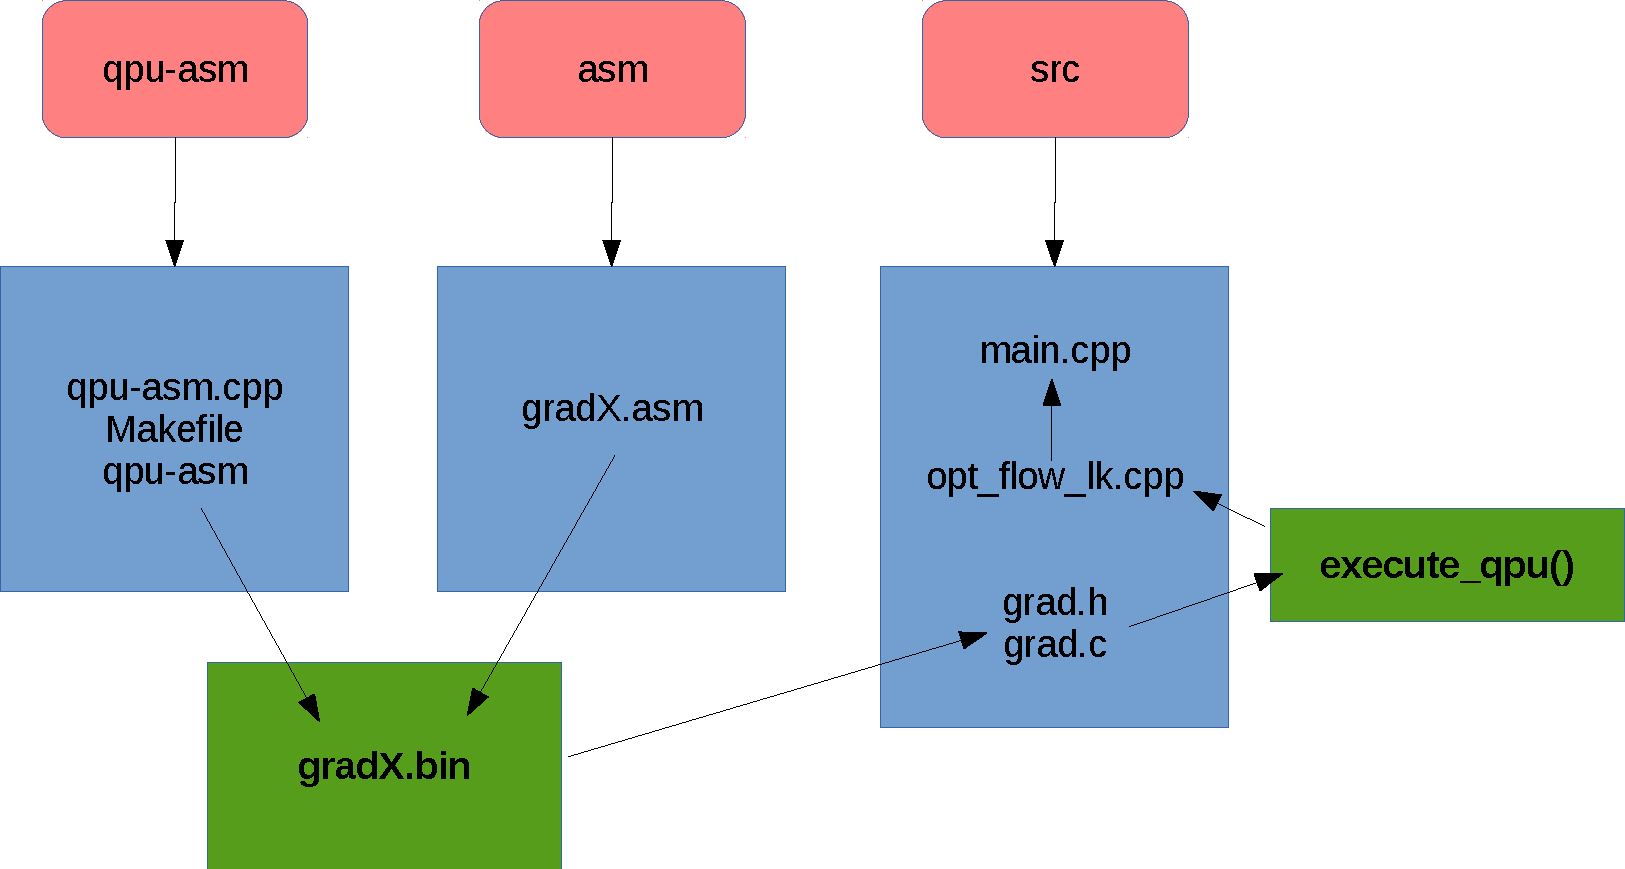
\includegraphics[scale=0.3]{images/projectResume.pdf}
\end{figure}

\end{frame}

%--------------------------------------------------------------------



%%%%%%%%%%%%%%%%%%%%%%%%%%%%%%%%%%%%%%%%%%%%%%%%%%%%%%%%%%%%%%%%%%%%%
%%%%%%%%%%%%%%%%%%%%%%%%%%%%%%%%%%%%%%%%%%%%%%%%%%%%%%%%%%%%%%%%%%%%%

\section{Résultats}

%%%%%%%%%%%%%%%%%%%%%%%%%%%%%%%%%%%%%%%%%%%%%%%%%%%%%%%%%%%%%%%%%%%%%

\subsection{Temps \& Précision}

%--------------------------------------------------------------------

\begin{frame}[fragile]{Temps pour 24 frames}

\lstset{style=CStyle,caption={Utilisation de la fonction OpenCV},label=}
\begin{lstlisting}
mean time per frame: 0.00538982 for 24 frames.
JSON file of vectors of each features at each frames can be found at: /home/pi/video/video_out/video_out_vectors.json

Video with vector representing optical flow has been written at : /home/pi/video/video_out/video_out_opt_flow_vectors.avi

**********************************************************************
**********************************************************************
All videos / frames of: /home/pi/video have been processed !
**********************************************************************
\end{lstlisting}

\lstset{style=CStyle,caption={Utilisation du VideoCore IV 3D},label=}
\begin{lstlisting}
mean time per frame: 0.0119438 for 24 frames.
JSON file of vectors of each features at each frames can be found at: /home/pi/video/video_out/video_out_vectors.json

Video with vector representing optical flow has been written at : /home/pi/video/video_out/video_out_opt_flow_vectors.avi

**********************************************************************
**********************************************************************
All videos / frames of: /home/pi/video have been processed !
**********************************************************************
\end{lstlisting}

\end{frame}

%--------------------------------------------------------------------

\begin{frame}{Précision pour la frame 1}

\begin{columns}

\begin{column}{0.2\textwidth}
\begin{tcolorbox}[tabgris,tabularx={|Y|}, boxrule=0.5pt, fontupper=\tiny, fontlower=\tiny, title=FRAME 1]
feature\\\hline\hline
1:\\
2:\\
3:\\
4:\\
5:\\
6:\\
7:\\
8:\\
9:\\
10:\\
11:\\
12:\\
13:\\
14:\\
15:\\
16:\\
17:\\
18:\\
19:\\
20:\\
21:\\
22:\\
23:\\
24:\\
25:\\
26:\\
27:\\
28:\\
29:\\
30:\\
\end{tcolorbox}
\end{column}

\begin{column}{0.4\textwidth}
\begin{tcolorbox}[tabjaune,tabularx={Y|Y}, boxrule=0.5pt, fontupper=\tiny, fontlower=\tiny, title=OpenCV]
$d_{y}$ & $d_{x}$\\\hline\hline
0.0529022 & 1.44458\\
0.0597687 & 1.52913\\
0.0342407 & 1.41058\\
0.112976 & 1.22267\\
0.0827942 & 1.44588\\
0.248459 & 1.40508\\
-0.015213 & 1.4809\\
0 & 0\\
0.0228882 & 1.63636\\
0.0141602 & 1.18526\\
0.168091 & 1.44987\\
0.13475 & 1.66971\\
0 & 0\\
0.00767517 & 1.44165\\
0 & 0\\
0.0722351 & 1.42871\\Temps
0.102554 & 1.21632\\
-0.010025 & 1.1138\\
0 & 0\\
0.0588074 & 1.37506\\
0 & 0\\
0 & 0\\
0 & 0\\
0 & 0\\
0 & 0\\
0 & 0\\
-0.0355682 & 1.50957\\
0 & 0\\
0 & 0\\
0 & 0
\end{tcolorbox}
\end{column}

\begin{column}{0.4\textwidth}
\begin{tcolorbox}[tabvert,tabularx={Y|Y}, boxrule=0.5pt, fontupper=\tiny, fontlower=\tiny, title=VideoCore IV 3D]
$d_{y}$ & $d_{x}$\\\hline\hline
0.051239  & 1.49907\\
0.0566864  & 1.49538\\
0.0485229  & 1.35619\\
0.117294  & 1.25969\\
0.0852509  & 1.44672\\
0.166031  & 1.45792\\
0.0622253  & 1.5038\\
0.0437317  & 1.45819\\
0.117691  & 1.69427\\
0.00265503  & 1.25769\\
0.241287  & 1.31388\\
0.139465  & 1.62927\\
0.129959  & 1.47935\\
0.12989  & 1.47667\\
0.0406952  & 1.49666\\
0.094986  & 1.3511\\
0.0591583  & 1.27177\\
0.0367737  & 1.13118\\
0.0540619  & 1.21773\\
0.158203  & 1.45867\\
0.0509186  & 1.89022\\
0.0492096  & 1.49521\\
0.295776  & 1.60911\\
0.17981  & 1.46049\\
0.0469666  & 1.3327\\
0.105698  & 1.47306\\
0.115067  & 1.43921\\
0.0691986  & 1.4396\\
0.0128326  & 1.17252\\
-0.0117493  & 1.12878
\end{tcolorbox}
\end{column}

\end{columns}

\end{frame}

%--------------------------------------------------------------------

%%%%%%%%%%%%%%%%%%%%%%%%%%%%%%%%%%%%%%%%%%%%%%%%%%%%%%%%%%%%%%%%%%%%%

\subsection{Perspectives}

%--------------------------------------------------------------------

\begin{frame}{Gestion des mouvements larges}

\begin{block}{Algorithme Pyramide}
\begin{itemize}
\item Entre 2 images successives
\item Pré-traitement de la première et de la seconde image
	\begin{itemize}
		\item Double convolution par un kernel gaussien $(3\times 3)$
			\begin{itemize}
				\item $(240\times 360)$ pixels à $(238\times 358)$ pixels
				\item $(238\times 358)$ pixels à $(236\times 356)$ pixels
			\end{itemize}
		\item Sélection pixel paire sur ligne paire -- $(118\times 178)$ pixels
	\end{itemize}
\item Applique les algorithmes précédents entre les deux images de $(118\times 178)$ pixels
\item Valeurs approchées de $d_{x}$ et $d_{y}$ pour chaque FEATURE
\item Reprise des algorithmes précédents sur les images $(240\times 360)$ pixels avec des valeurs initiales différentes
\end{itemize}
\end{block}

\end{frame}

%--------------------------------------------------------------------



%%%%%%%%%%%%%%%%%%%%%%%%%%%%%%%%%%%%%%%%%%%%%%%%%%%%%%%%%%%%%%%%%%%%%
%%%%%%%%%%%%%%%%%%%%%%%%%%%%%%%%%%%%%%%%%%%%%%%%%%%%%%%%%%%%%%%%%%%%%
\section{Conclusion}

%--------------------------------------------------------------------

\begin{frame}{Conclusion}
\boitebleue{
	Démonstration sur une courte vidéo issue de la RaspiCam de iBubble.
}
\end{frame}

%--------------------------------------------------------------------



%\section{Aperçu global}
%
%\begin{frame}{Aperçu global}
%Texte normal \alert{Texte Alert}  \exemple{Texte exemple} \emph{Texte emphase}
%
%\begin{columns}
%
%\begin{column}{0.5\textwidth}
%\begin{block}{Bloc simple}
%\begin{itemize}
%\item Premier point
%\end{itemize}
%\end{block}
%
%\begin{exampleblock}{Bloc exemple}
%\begin{itemize}
%\item Premier point
%\end{itemize}
%\end{exampleblock}
%
%\begin{alertblock}{Bloc alert}
%\begin{itemize}
%\item Premier point
%\end{itemize}
%\end{alertblock}
%
%\end{column}
%
%\begin{column}{0.5\textwidth}
%\boiteviolette{
%Une boite violette
%}
%
%\boiteorange{
%Une boite orange
%}
%
%\boitegrise{
%Une boite grise
%}
%
%
%
%\begin{tcolorbox}[tabvert,tabularx={X||Y|Y|Y|Y||Y}, boxrule=0.5pt, title=Mon tableau des prix]
%Couleur & Prix 1  & Prix 2  & Prix 3 \\\hline\hline
%Rouge   & 10.00   & 20.00   &  30.00 \\\hline
%Vert    & 20.00   & 30.00   &  40.00  \\\hline
%Bleu    & 30.00   & 40.00   &  50.00 \\\hline\hline
%Orange  & 60.00   & 90.00   & 120.00
%\end{tcolorbox}
%
%\end{column}
%
%\end{columns}
%\end{frame}
%
%
%
%
%\section{Les blocs}
%
%\begin{frame}{Les blocs}
%
%\begin{block}{Bloc simple}
%\begin{itemize}
%\item Premier point
%\item Second point
%\item Troisième point
%\end{itemize}
%\end{block}
%
%\begin{exampleblock}{Bloc exemple}
%\begin{itemize}
%\item Premier point
%\item Second point
%\item Troisième point
%\end{itemize}
%\end{exampleblock}
%
%\begin{alertblock}{Bloc alert}
%\begin{itemize}
%\item Premier point
%\item Second point
%\item Troisième point
%\end{itemize}
%\end{alertblock}
%\end{frame}
%
%
%\section{Les bo\^ites}
%
%\begin{frame}{Les boites}
%
%\begin{columns}
%
%\begin{column}{0.5\textwidth}
%\boitejaune{
%Ceci est \\
%une boite jaune
%}
%
%\boiteorange{
%Ceci est \\
%une boite orange
%}
%
%\boitemarron{
%Ceci est \\
%une boite marron
%}
%\end{column}
%
%\begin{column}{0.5\textwidth}
%\boiteviolette{
%Ceci est \\
%une boite violette
%}
%
%\boitebleue{
%Ceci est \\
%une boite bleue
%}
%
%\boitegrise{
%Ceci est \\
%une boite grise
%}
%
%\end{column}
%
%\end{columns}
%
%
%\end{frame}
%
%
%
%\section{Les listes}
%	\subsection{Liste à item}
%
%\begin{frame}{Titre de la frame}
%
%	\begin{itemize}
%		\item premier élément de liste,
%		\item deuxième élément de liste,
%		\item troisième élément de liste.
%	\end{itemize}
%\end{frame}
%
%		\subsection{Liste énumérative}
%\begin{frame}{Titre de la frame}
%	\begin{enumerate}
%		\item élément de liste numéro 1,
%		\item élément de liste numéro 2,
%		\item élément de liste numéro 3.
%	\end{enumerate}
%\end{frame}
%
%
%		\subsection{Liste descriptive}
%\begin{frame}{Titre de la frame}
%	\begin{description}
%		\item [Thème de présentation : ] ces thèmes sont en fait...
%		\item [Thème de couleur : ] gère tout ce qui est couleur...
%		\item [Thème de police : ] s'occupe de tout ce qui est police, gras...
%		\item [Thème interne : ] s'occupe de l'apparence des éléments...
%	\end{description}
%\end{frame}
%
%
%
%\section{Le texte}
%
%\begin{frame}{Titre de la frame}
%
%Voici du texte normal
%
%\alert{Voici du texte \texttt{alert}}
%
%\exemple{Voici du texte \texttt{exemple}}
%
%\emph{Voici du texte \texttt{emphase}}
%
%\end{frame}
%
%
%\section{Les tableaux}
%
%\begin{frame}{Tableaux}
%
%% merci: http://tex.stackexchange.com/questions/112343/beautiful-table-samples
%
%\begin{tcolorbox}[tabjaune,tabularx={X||Y|Y|Y|Y||Y}, boxrule=0.5pt]
%Couleur & Prix 1  & Prix 2  & Prix 3   & Prix 4   & Prix 5 \\\hline\hline
%Rouge   & 10.00   & 20.00   &  30.00   &  40.00   & 100.00 \\\hline
%Vert    & 20.00   & 30.00   &  40.00   &  50.00   & 140.00 \\\hline
%Bleu    & 30.00   & 40.00   &  50.00   &  60.00   & 180.00 \\\hline\hline
%Orange  & 60.00   & 90.00   & 120.00   & 150.00   & 420.00
%\end{tcolorbox}
%
%\begin{tcolorbox}[tabvert,tabularx={X||Y|Y|Y|Y||Y}, boxrule=0.5pt, title=Mon tableau des prix]
%Couleur & Prix 1  & Prix 2  & Prix 3   & Prix 4   & Prix 5 \\\hline\hline
%Rouge   & 10.00   & 20.00   &  30.00   &  40.00   & 100.00 \\\hline
%Vert    & 20.00   & 30.00   &  40.00   &  50.00   & 140.00 \\\hline
%Bleu    & 30.00   & 40.00   &  50.00   &  60.00   & 180.00 \\\hline\hline
%Orange  & 60.00   & 90.00   & 120.00   & 150.00   & 420.00
%\end{tcolorbox}
%
%\end{frame}
%
%
%\begin{frame}{Tableaux}
%
%% merci: http://tex.stackexchange.com/questions/112343/beautiful-table-samples
%
%\begin{tcolorbox}[tabgris,tabularx={X||Y|Y|Y|Y||Y}, boxrule=0.5pt]
%Couleur & Prix 1  & Prix 2  & Prix 3   & Prix 4   & Prix 5 \\\hline\hline
%Rouge   & 10.00   & 20.00   &  30.00   &  40.00   & 100.00 \\\hline
%Vert    & 20.00   & 30.00   &  40.00   &  50.00   & 140.00 \\\hline
%Bleu    & 30.00   & 40.00   &  50.00   &  60.00   & 180.00 \\\hline\hline
%Orange  & 60.00   & 90.00   & 120.00   & 150.00   & 420.00
%\end{tcolorbox}
%
%\begin{tcolorbox}[taborange,tabularx={X||Y|Y|Y|Y||Y}, boxrule=0.5pt, title=Mon tableau des prix]
%Couleur & Prix 1  & Prix 2  & Prix 3   & Prix 4   & Prix 5 \\\hline\hline
%Rouge   & 10.00   & 20.00   &  30.00   &  40.00   & 100.00 \\\hline
%Vert    & 20.00   & 30.00   &  40.00   &  50.00   & 140.00 \\\hline
%Bleu    & 30.00   & 40.00   &  50.00   &  60.00   & 180.00 \\\hline\hline
%Orange  & 60.00   & 90.00   & 120.00   & 150.00   & 420.00
%\end{tcolorbox}
%
%\end{frame}
%
%
%
%\section{Les images}
%
%\begin{frame}{Titre de la frame}
%
%\begin{figure}
%\centering
%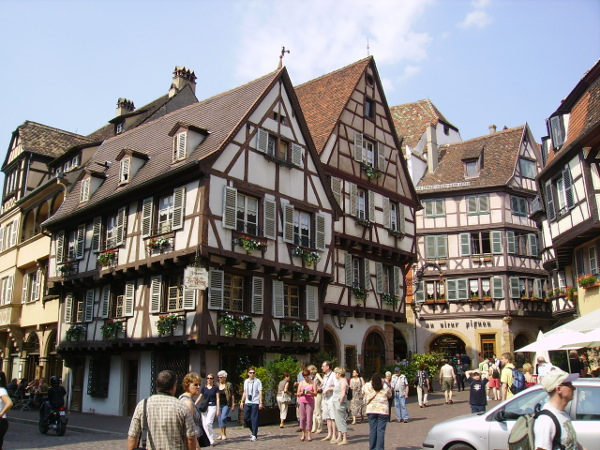
\includegraphics[scale=0.5]{images/architecturebretonne_wikipedia.jpg}
%\caption{Éléments d'architecture bretonne typique du Sud de la France. (\href{http://commons.wikimedia.org/wiki/File:Colmar_-_Alsace.jpg}{Wikipédia.fr} CC-By-Sa)}
%\end{figure}
%
%\end{frame}



\end{document}
